\Chapter{Configurazione Sperimentale}

Per effettuare gli esperimenti ho avuto la possibilità di utilizzare un \textbf{framework sperimentale} sviluppato dall'ingegner \hlight{Marco Cantone} ~\cite{MarcoCantone}, \textbf{correlatore di questa tesi}. Il cuore del framework risiedeva nella sua capacità di \textbf{astrarre la complessità tipica degli esperimenti di deep learning} attraverso una struttura di configurazione \textbf{gerarchica} e \textbf{intuitiva}. Ogni aspetto cruciale del processo, dal \textbf{preprocessing} dei dati alla \textbf{definizione dell'architettura}, dagli \textbf{iperparametri di training} alle \textbf{metriche di valutazione}, trovava una precisa collocazione nel file \textbf{YAML}.

Uno dei maggiori vantaggi di questo approccio emergeva nella \textbf{fase di validazione incrociata delle ipotesi}. La possibilità di confrontare direttamente diverse varianti architetturali, mantenendo invariati tutti gli altri parametri, ha permesso di isolare con precisione l'impatto di ciascuna scelta progettuale.


Sebbene il framework fornisse una struttura organizzata per gli esperimenti, \textbf{non era dotato di sistemi intelligenti in grado di verificare automaticamente la coerenza logica delle configurazioni}. Spettava quindi a me, durante la definizione dei parametri nel file YAML, assicurarmi che le scelte fossero \textbf{compatibili} tra loro e adatte al contesto. Ad esempio, se impostavo un'architettura progettata per input volumetrici, dovevo verificare manualmente che anche le trasformazioni di preprocessing (come il random padding o il resizing) fossero configurate per operare su tre dimensioni, evitando incongruenze che avrebbero compromesso l'addestramento. 

\begin{figure}[H]
  \centering
  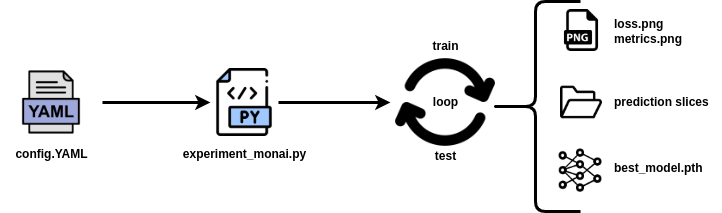
\includegraphics[width=\textwidth]{figures/Untitled Diagram.drawio.png}
\end{figure}


Allo stesso modo, quando sperimentavo ottimizzatori diversi, dovevo prestare attenzione alla scelta del \textbf{learning rate} e dello \textbf{scheduler}, poiché valori troppo aggressivi potevano \textbf{destabilizzare il training}, mentre quelli troppo conservativi \textbf{rallentavano inutilmente la convergenza}. 

Questo processo richiedeva una costante \textbf{analisi degli errori}: se un esperimento falliva o produceva risultati insoliti, dovevo riesaminare la configurazione YAML per identificare possibili discrepanze, come \textbf{dimensioni di crop incompatibili} con la \textbf{risoluzione del volume} o \textbf{parametri di augmentazione eccessivamente distorti}. La mancanza di validazione automatica ha reso il lavoro più impegnativo, ma mi ha spinto a \textbf{sviluppare una profonda comprensione delle dipendenze tra i vari componenti del sistema}.


\Section{Il file di configurazione YAML}
Il file di configurazione YAML è organizzato in \textbf{sezioni logiche} che definivano ogni aspetto del processo di \textbf{addestramento} e \textbf{valutazione}. Di seguito, analizziamo le componenti principali del file, suddividendolo in sottoinsiemi funzionali.

\Subsection{Struttura generale}
Il file YAML è organizzato in 6 sezioni principali:

\begin{code}{yaml}
# Esempio di struttura generale
TRAINING:
  # parametri di addestramento
TRAIN_TRANSFORM:
  # trasformazioni per il training
TEST_TRANSFORM:
  # trasformazioni per il test
MODEL:
  # architettura del modello
LOSS:
  # funzione di loss
OPTIMIZER:
  # ottimizzatore
\end{code}

\Subsection{Configurazione del training}
La sezione \texttt{TRAINING} definiva i parametri fondamentali:

\begin{code}{yaml}
TRAINING:
  workspace: /path/to/experiment_results
  dataset_root: /path/to/dataset
  valid_size: 0.1  # 10% validation set
  test_size: 0.1   # 10% test set
  train_batch_size: 4
  test_batch_size: 1 
  num_workers: 8    # thread per data loading
  device: cuda:0    # GPU da utilizzare
  epochs: 50        # numero di epoche
  roi_size: [256, 256, 32]  # dimensione regioni di interesse
\end{code}

\Subsection{Trasformazioni dei dati}

Le sezioni \texttt{TRAIN\_TRANSFORM} e \texttt{TEST\_TRANSFORM} specificavano il preprocessing:

\begin{code}{yaml}
TRAIN_TRANSFORM:
  - class: monai.transforms.LoadImaged
    params:
      keys: ['post_2', 'breast']
  - class: monai.transforms.RandSpatialCropSamplesd
    params:
      keys: ['img', 'seg']
      num_samples: 4
      roi_size: [512, 512, 8]
\end{code}


\Subsection{Definizione del modello}
La sezione \texttt{MODEL} configurava l'architettura della rete:

\begin{code}{yaml}
MODEL:
  class: monai.networks.nets.Unet
  params:
    channels: [16, 32, 64]  # canali per ogni livello
    in_channels: 1          # canali input
    out_channels: 2         # canali output
    norm: INSTANCE          # normalizzazione
    spatial_dims: 3         # dimensione spaziale
    strides: [2, 2, 2]      # stride dei livelli
\end{code}


\Subsection{Ottimizzazione e loss}
Le sezioni \texttt{LOSS} e \texttt{OPTIMIZER} controllavano l'addestramento, includendo la funzione di loss e l'ottimizzatore:


\begin{code}{yaml}
LOSS:
  class: monai.losses.DiceFocalLoss
  params:
    weight_dice: 0.7
    weight_ce: 0.3

OPTIMIZER:
  class: torch.optim.AdamW
  params:
    lr: 1e-3               # learning rate
    weight_decay: 1e-3      # regolarizzazione
\end{code}


\Subsection{Post-processing e valutazione}
Le sezioni finali gestivano la valutazione:

\begin{code}{yaml}
METRIC:
  class: monai.metrics.DiceMetric
  params:
    include_background: false
    reduction: mean

POST_PRED:                                                                              
  - class: monai.transforms.AsDiscrete
    params:
      argmax: true
      to_onehot: 2

POST_LABEL:                                                                                 
  - class: monai.transforms.AsDiscrete
    params:
      to_onehot: 2
\end{code}



\Section{Gestione del Logging}

Per ogni esperimento è stato adottato un sistema di \textbf{logging automatico} organizzato in modo da raccogliere tutti gli output generati in una \textbf{cartella dedicata}, con l’obiettivo di garantire tracciabilità, riproducibilità e analisi approfondita dei risultati.

%Struttura delle cartelle
La struttura delle cartelle seguiva uno schema gerarchico, con una cartella principale per ogni esperimento, identificata da un nome univoco basato sulla data e sull'ora di inizio. All'interno di questa cartella, venivano create sottocartelle
per ogni fase del processo di addestramento e valutazione, consentendo una facile navigazione e gestione dei risultati. Ad esempio, la struttura poteva apparire come segue:\\
\begin{minipage}{\textwidth}
\begin{code}{bash}
+-- exp_i/
|   +-- log.txt
|   +-- loss_curve.png
|   +-- metric_curve.png
|   +-- best_model.pth
|   +-- predictions/
|       +-- case_001/
|       |   +-- slice_01.png
|       |   +-- slice_02.png
|       |   +-- ...
|       +-- case_002/
|       |   +-- slice_01.png
|       |   +-- ...
|       +-- ...
\end{code}
\end{minipage}
\\


Ogni cartella conteneva le seguenti informazioni:

\begin{itemize}
\item Un file \texttt{log.txt} contenente tutte le stampe console (\texttt{print}) prodotte durante il training. In questo file venivano riportati:
\begin{itemize}
\item la \textbf{loss di training} e \textbf{validazione} per epoca;
\item le \textbf{metriche di valutazione} (es. \textbf{Dice score});
\item eventuali \textbf{messaggi diagnostici}.
\end{itemize}
\item Due \textbf{grafici} in formato immagine (\texttt{.png}):
\begin{itemize}
    \item il grafico della \textbf{curva della loss} per epoca;
    \item il grafico della \textbf{metrica} per epoca.
\end{itemize}

\item Il file del \textbf{modello salvato} (\texttt{.pth}), che rappresenta lo \textbf{stato della rete al miglior checkpoint}.

\item Una sottocartella \texttt{predictions/} contenente, per ogni caso del \textbf{test set}, le \textbf{immagini salvate slice per slice}. Ogni immagine mostrava sovrapposte:
\begin{itemize}
    \item \textbf{l’immagine originale della MRI dell'i-esima slice}
    \item la \textbf{ground truth} dell'i-esima slice
    \item la \textbf{predizione generata dal modello} dell'i-esima slice
\end{itemize}

\end{itemize}

Questa struttura ha permesso non solo di \textbf{monitorare l’andamento dell’addestramento}, ma anche di effettuare \textbf{confronti qualitativi tra modelli diversi} e analizzare visivamente i punti di \textbf{forza} e \textbf{debolezza} della rete. Inoltre, la separazione per cartelle ha reso semplice la gestione di esperimenti multipli e il confronto sistematico tra diverse configurazioni di training.